
\documentclass{beamer}

\usetheme{default}

\usepackage{subcaption}
\usepackage{graphicx}
\begin{document}

\title{Quick results}
\author{Pierre Marrec}
\date{\today}

\begin{frame}
    \titlepage
\end{frame}

\begin{frame}
    \frametitle{Introduction}

\begin{itemize}
    \item short $\leq$ 15 min
    \item long $>$ 15 min
\end{itemize}
\begin{table}
    \centering
    \begin{tabular}{|c|c|c|c|}
        \hline
        type & long & short & total \\
        \hline
        route & 540 & 5 & 545 \\
        piste & 150 & 71 & 221 \\
        home & 124 & 1 & 125 \\
        clm & 73 & 1 & 74 \\
        total & 887 & 78 & 965 \\
        \hline
    \end{tabular}
\end{table}

\end{frame}

% Add more frames for your presentation




\begin{frame}
    \begin{figure}
        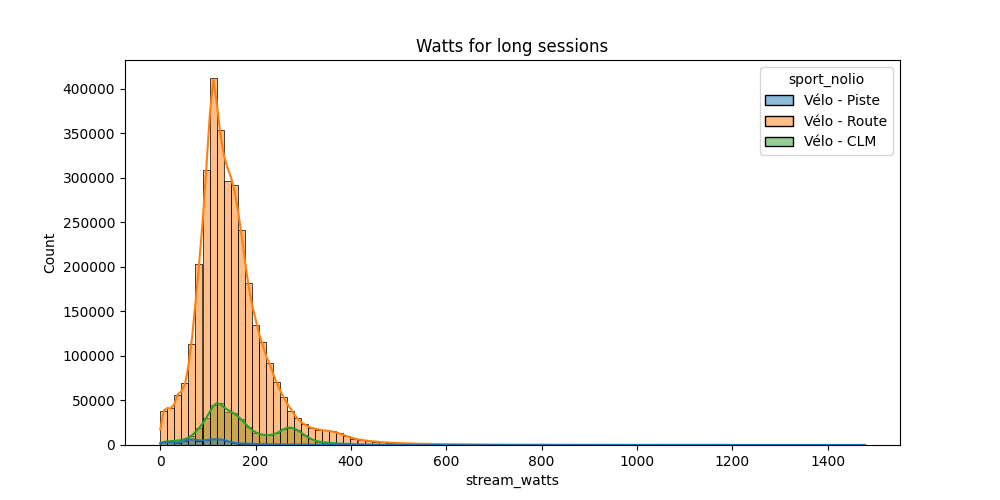
\includegraphics[width=\textwidth]{../ppr/watts_long.png}
    \end{figure}
\end{frame}

\begin{frame}
    \begin{figure}
        \begin{subfigure}{0.7\textwidth}
            \centering
            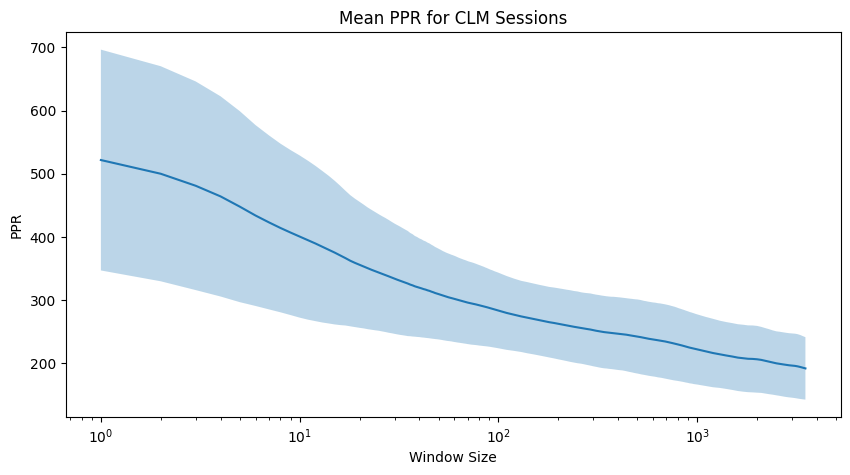
\includegraphics[width=\textwidth]{../ppr/ppr_clm_mean.png}
            \caption{CLM}
        \end{subfigure}
        \begin{subfigure}{0.7\textwidth}
            \centering
            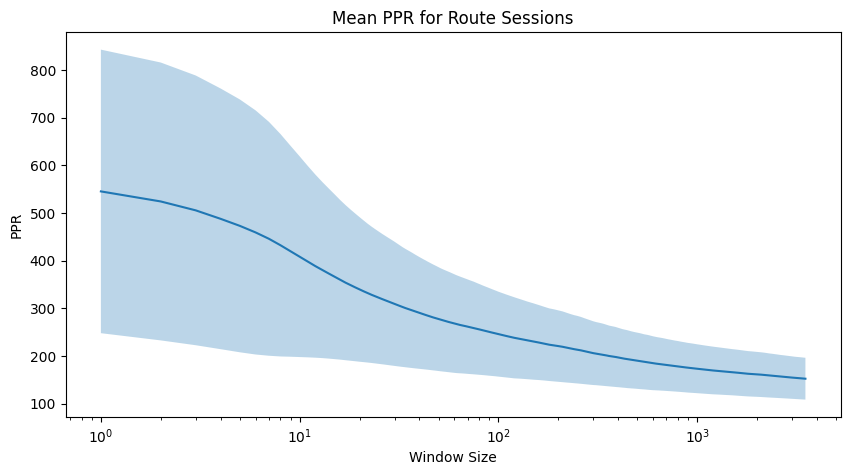
\includegraphics[width=\textwidth]{../ppr/ppr_route_mean.png}
            \caption{Route}
        \end{subfigure}
    \end{figure}
\end{frame}

\begin{frame}
    \begin{figure}
        \centering
        \begin{subfigure}{0.7\textwidth}
            \centering
            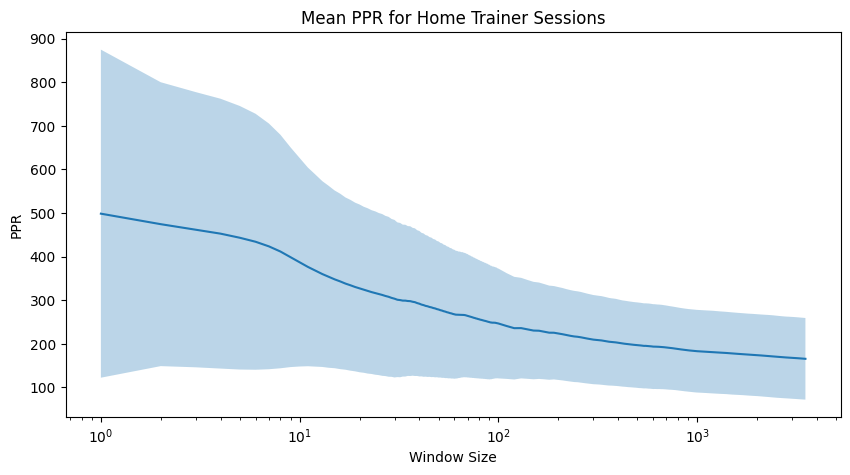
\includegraphics[width=\textwidth]{../ppr/ppr_home_mean.png}
            \caption{HomeTrainer}
        \end{subfigure}

        \begin{subfigure}{0.7\textwidth}
            \centering
            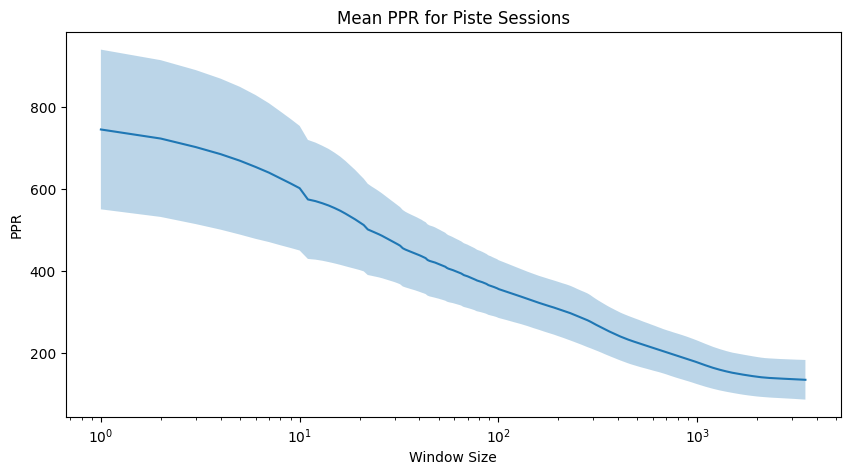
\includegraphics[width=\textwidth]{../ppr/ppr_piste_mean.png}
            \caption{Piste}
        \end{subfigure}

    \end{figure}
\end{frame}


\begin{frame}
    %subfigure of 4
    \begin{figure}
        \centering
        \begin{subfigure}{0.7\textwidth}
            \centering
            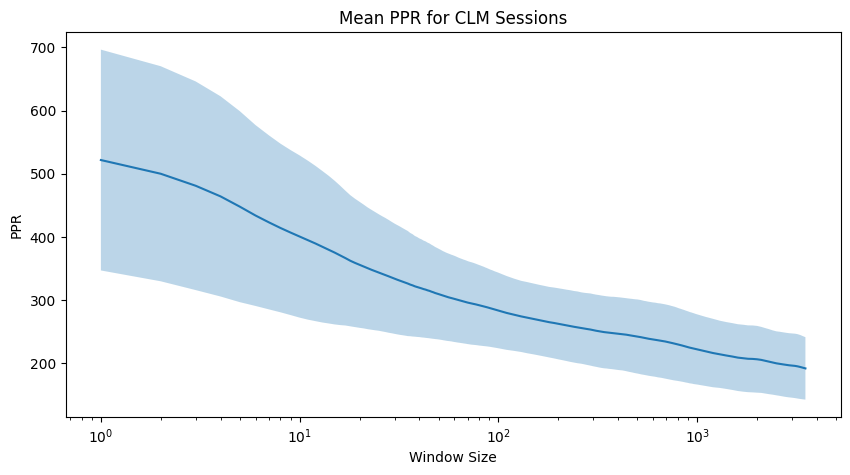
\includegraphics[width=\textwidth]{../ppr/ppr_clm.png}
            \caption{CLM}
        \end{subfigure}
        \begin{subfigure}{0.7\textwidth}
            \centering
            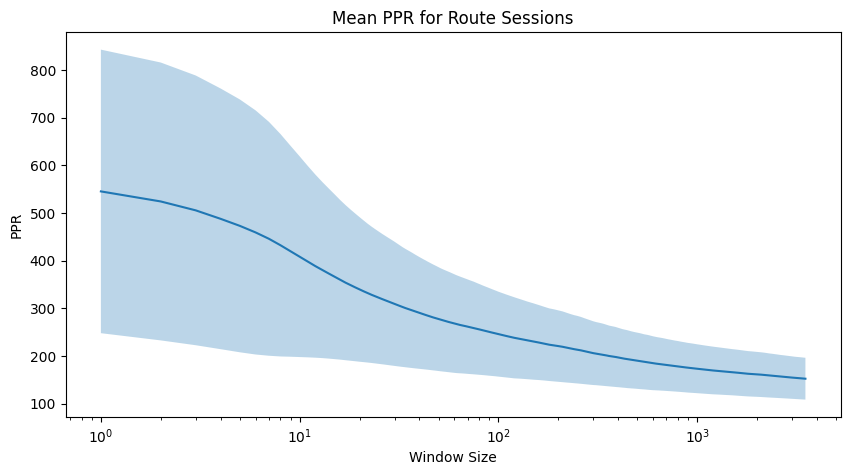
\includegraphics[width=\textwidth]{../ppr/ppr_route.png}
            \caption{Route}
        \end{subfigure}
    \end{figure}
\end{frame}
\begin{frame}

    \begin{figure}
        \centering
        \begin{subfigure}{0.7\textwidth}
            \centering
            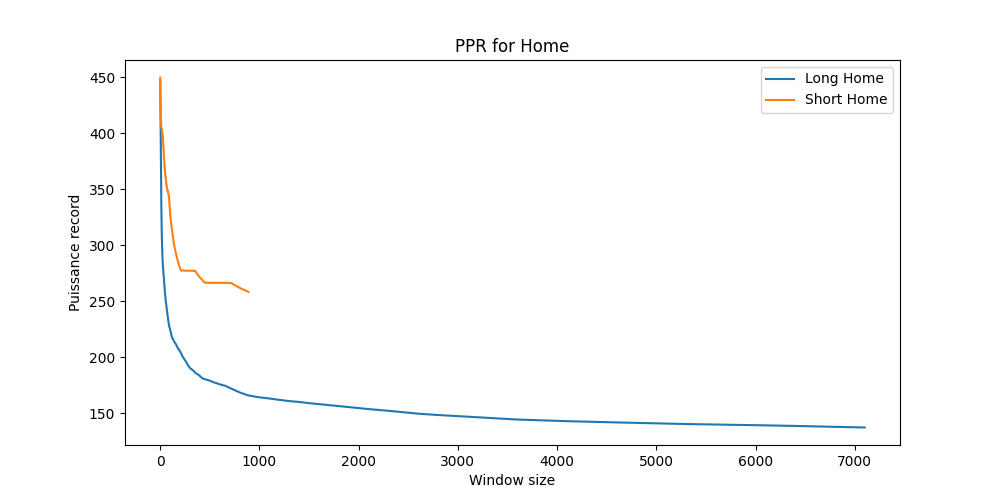
\includegraphics[width=\textwidth]{../ppr/ppr_home.png}
            \caption{HomeTrainer}
        \end{subfigure}

        \begin{subfigure}{0.7\textwidth}
            \centering
            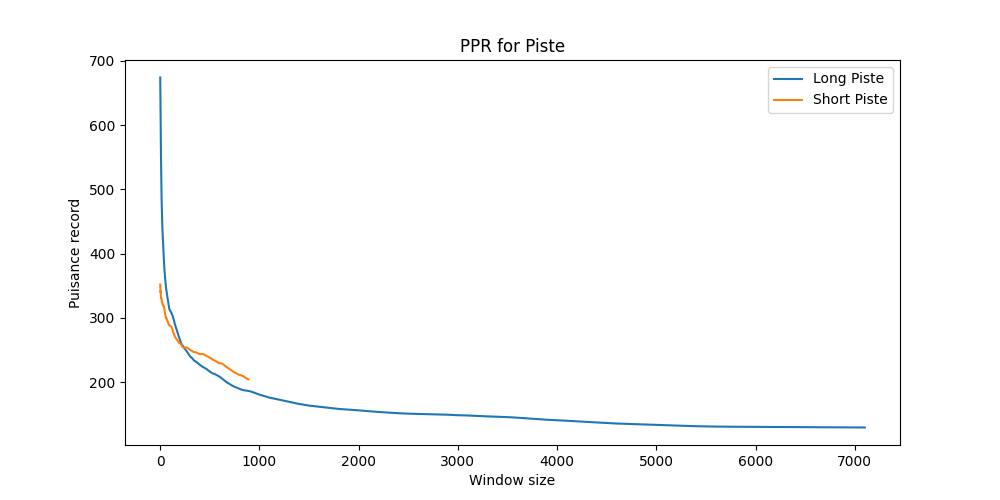
\includegraphics[width=\textwidth]{../ppr/ppr_piste.png}
            \caption{Piste}
        \end{subfigure}

    \end{figure}
\end{frame}


% same with log at the end

\begin{frame}
    \begin{figure}
        \centering
        \begin{subfigure}{0.7\textwidth}
            \centering
            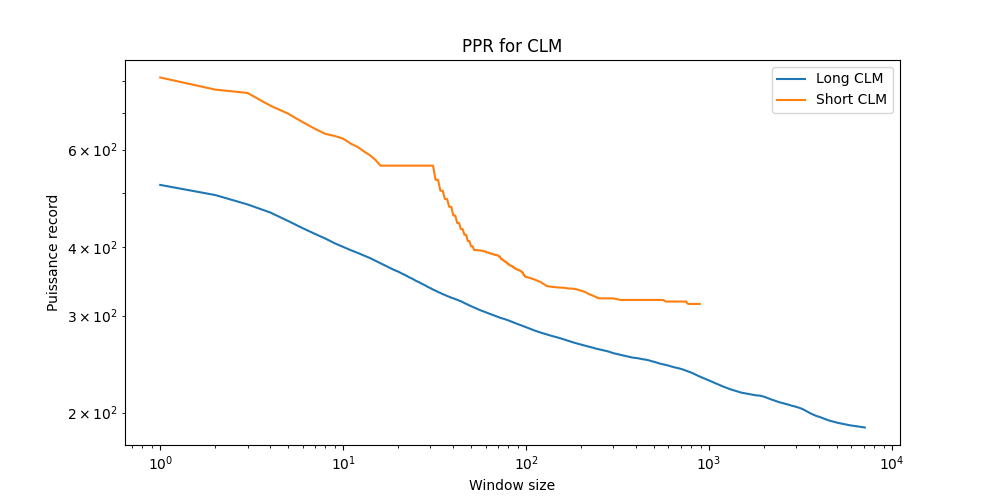
\includegraphics[width=\textwidth]{../ppr/ppr_clm_log.png}
            \caption{CLM}
        \end{subfigure}
        \begin{subfigure}{0.7\textwidth}
            \centering
            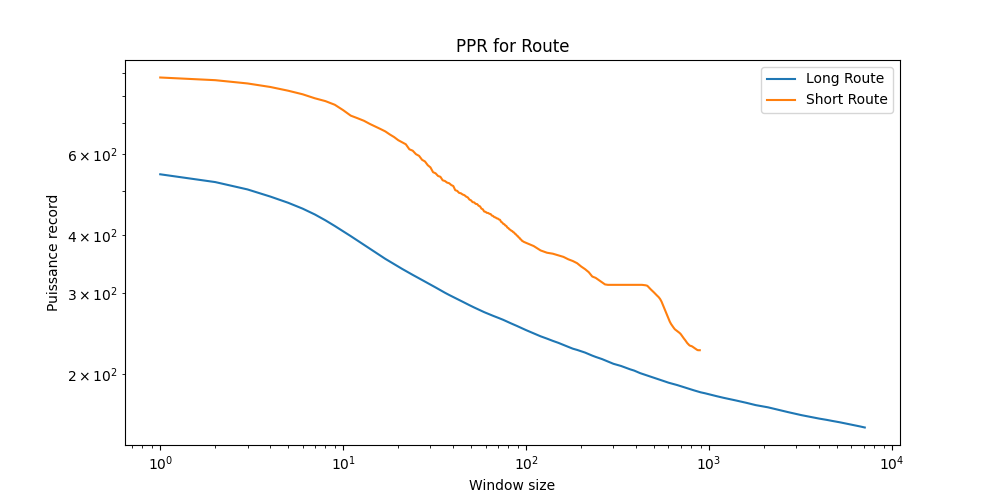
\includegraphics[width=\textwidth]{../ppr/ppr_route_log.png}
            \caption{Route}
        \end{subfigure}
    \end{figure}
\end{frame}

\begin{frame}

    \begin{figure}
        \centering
        \begin{subfigure}{0.7\textwidth}
            \centering
            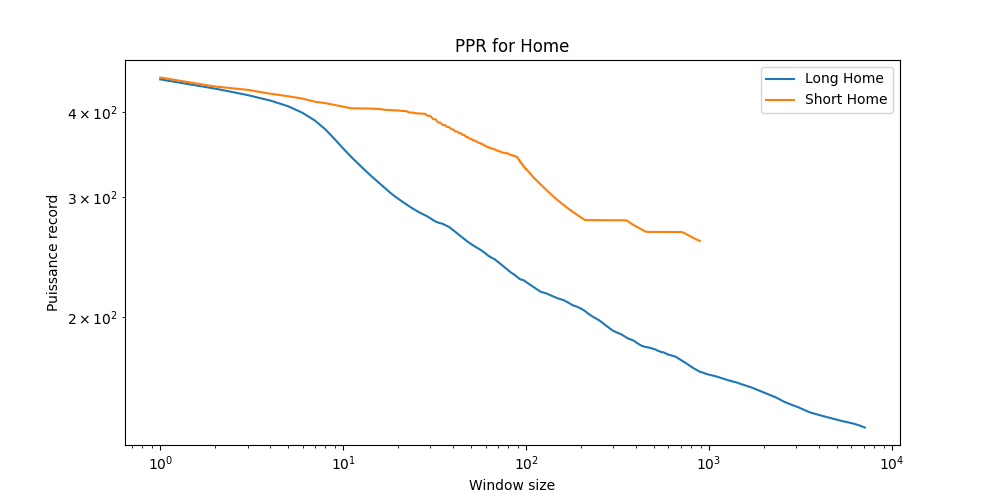
\includegraphics[width=\textwidth]{../ppr/ppr_home_log.png}
            \caption{HomeTrainer}
        \end{subfigure}

        \begin{subfigure}{0.7\textwidth}
            \centering
            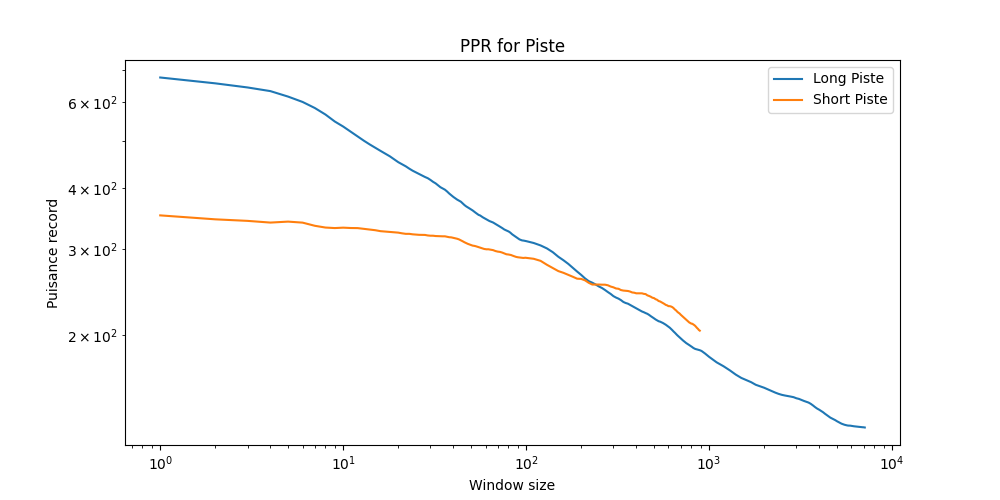
\includegraphics[width=\textwidth]{../ppr/ppr_piste_log.png}
            \caption{Piste}
        \end{subfigure}

    \end{figure}
\end{frame}


\begin{frame}
    
    \begin{figure}
        
        \begin{subfigure}{0.7\textwidth}
            \centering
            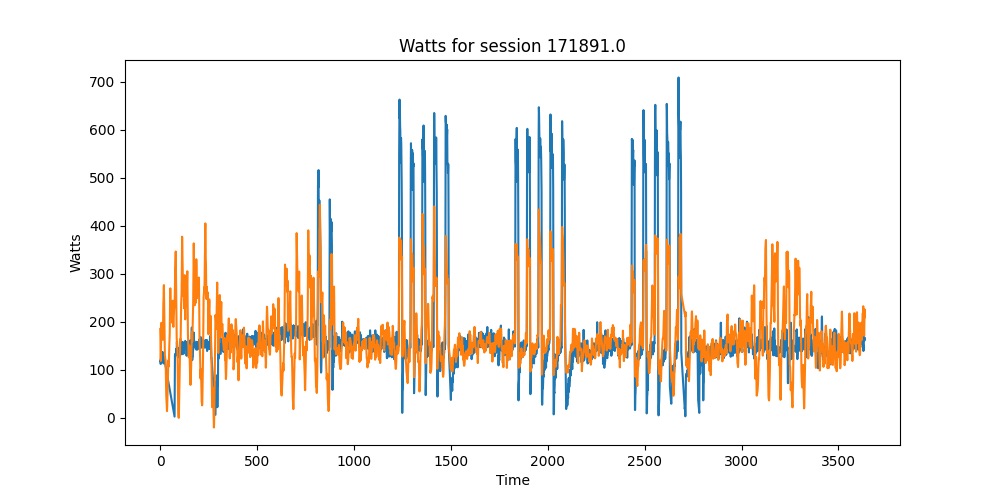
\includegraphics[width=\textwidth]{../reconstruction/watts_171891.0.png}
            \caption{Watts and FFT reconstruction
            }
        \end{subfigure}
        \begin{subfigure}{0.7\textwidth}
            \centering
            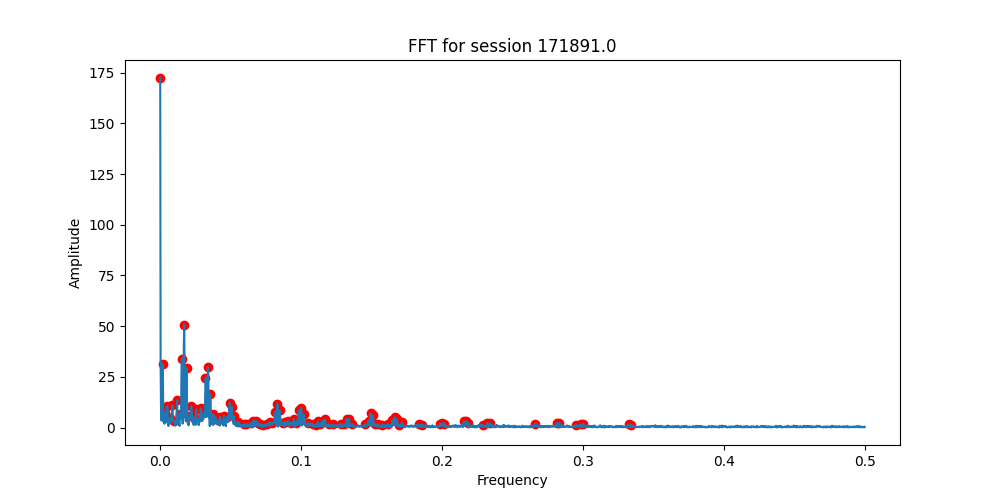
\includegraphics[width=\textwidth]{../reconstruction/fft_171891.0.png}
            \caption{FFT of the signal}
        \end{subfigure}

    \end{figure}


\end{frame}

\end{document}